\begin{exo}
	On considère l'arbre de probabilités ci-dessous représentant une situation aléatoire mettant en jeu deux événements $A$ et $B$.

	\begin{center}
		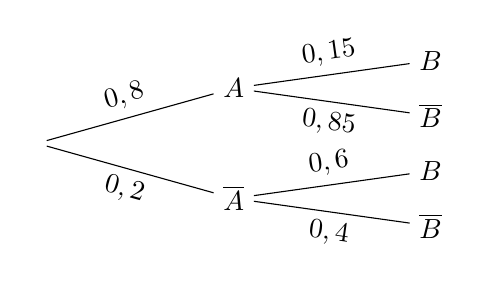
\begin{tikzpicture}[grow=right, sloped, level distance=2.5cm, level 1/.style={sibling distance=1.4cm}, level 2/.style={sibling distance=0.7cm}]
			\node {}
			child {node {$\overline{A}$}
					child {node {$\overline{B}$} edge from parent node[below] {$0,4$}}
					child {node {$B$} edge from parent node[above] {$0,6$}}
					edge from parent node[below] {$0,2$}
				}
			child {node {$A$}
					child {node {$\overline{B}$} edge from parent node[below] {$0,85$}}
					child {node {$B$} edge from parent node[above] {$0,15$}}
					edge from parent node[above] {$0,8$}
				};

		\end{tikzpicture}
	\end{center}

	\begin{enumerate}
		\item Par lecture directe sur l'arbre, donner les valeurs des probabilités suivantes :
		      \[
			      P(A)\ ,\ P_{A}(\overline{B})\ \text{ et }\ P_{\overline{A}}(B)
		      \]

		\item Calculer la probabilité des événements :
		      \[
				  A \cap B\ \text{ et }\ \bar{A} \cap B
		      \]

	\end{enumerate}
\end{exo}
